\chapter{ARTIFICIAL INTELLIGINCE (AI)}

Artificial Intelegence (AI) adalah cabang ilmu komputer yang mensimulasikan kecerdasan yang dimiliki oleh manusia yang diimplementasikan kedalam suatu program komputer, kecerdasan buatan adalah aktivitas mesin yang menampilkan prilaku yang dianggap hampir menyerupai kecerdasan yang dimiliki oleh manusia, sehingga bisa dikatakan AI merupakan sistem atau program kompute yang mampu melakukan pekerjaan dan memutuskan sesuatu seperti layaknya manusia.
AI juga merupakan tekhnologi yang memungkinkan mesin bisa mengerti apa yang pengguna inginkan dan butuhkan, misalnya untuk menciptakan mesin yang dapat menidentifikas suara dan mampu memberikan \textit{return} atau timbal balik dari mesin tersebut.


\section{Revolusi Industri 4.0 dan Artificial Intelegence}
Revolusi industri terjadi pertama kali di Inggris merupakan revolusi ekonomi. Corak perekonomian Inggris yang semula agraris berubah menjadi industri. Diantara ciri-cirinya adalah status sosial sangat dipengaruhi oleh luasnya kepemilikan tanah. Saat itu cara membuat barang juga masih konvensional yaitu mengandalkan tenaga manusia dan tenaga hewan. Pembuatan barang juga masih dikerjakan di rumah-rumah belum dilakukan di pabrik.
pada akhir abad ke-17, pembuatan (manufaktur) dikerjakan di rumah-rumah penduduk dengan menggunakan manual tangan atau menggunakan manual tangan atau menggunakan mesin sederhan. oleh sebab itu kemampuan menghasilkan barang masih terbatas.
\begin{enumerate}
  \item \textbf{Revolusi Industri 1.0} \\
     
  \item \textbf{Machine Learning}  \\
    Istiah \textit{mechine learning}  pertama kali dikemukakan oleh beberapa ilmuan matematika seperti Adren Marie Lagandrie, Thomas Bayes dan Andrey Mrkov pada tahun 1920-an dengan mengemukakan dasar-dasar \textit{mechine learning} dan konsepnya. sejak saat itu ML banyak yang mengembangkan. salah satu contoh dari penerapan ML yang cukup terkenal adalah \textit{deep blue} yang dibuat oleh IBM pada tahun 1996.
    Teknologi \textit{mechine learning}  adalah mesin yang dikembangkan untuk bisa belajar dengan sendirinya tanpa arahan dari pengguna atau \textit{user}, pembeljaran \textit{mechine learning}  dikembangkan berdasarkan disiplin ilmu lainya seperti statistika, matematika dan data mining sehingga mesin dapat belajar dengan menganalisis data tanpa perlu di program ulang atau diperintah.
    untuk bisa mengoprasikan \textit{mechine learning} secara optimal terdapat 3 metode yaitu: 
    \begin{figure} [ht] \centering
      % Nama dari file gambar yang diinputkan
      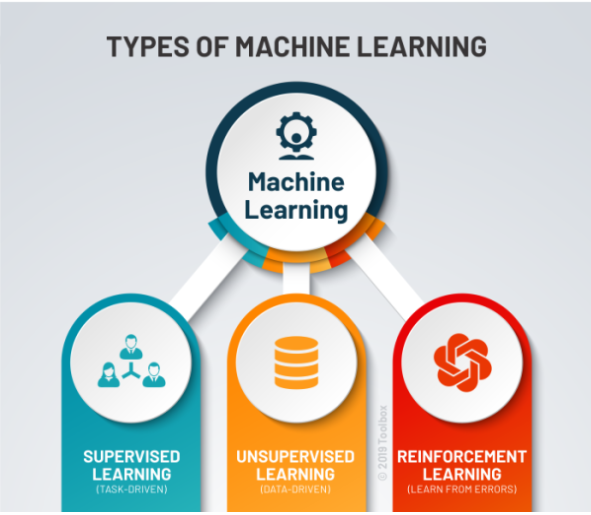
\includegraphics[scale=0.9]{gambar/metode_ML.png}
      % Keterangan gambar yang diinputkan
      \caption{tiga metode atau tipe mechine learning (Sumber: ekrut.com)}
      % Label referensi dari gambar yang diinputkan
      \label{fig:MechineLearning}
    \end{figure}
    \begin{enumerate}[nolistsep]
      \item \textit{\textbf{Supervised Learning}}\\
        Metode supervised learning dilakukan dengan pemberian label pada dataset  yang digunakan oleh machine learning dan diklasifikasikan oleh pengembang dengan memungkinkan algoritma melihat tingkat akurasi kinerjanya. Pengawasan machine learning dalam metode ini dilakukan oleh data berlabel yang nantinya membuat machine learning mempelajari apa hubungan dan ketergantungan antar data.
        Cara kerja metode ini adalah memasukkan informasi sebagai input dan data berlabel sebagai hasil atau output. Input dalam machine learning pinjaman bank misalnya dapat berupa data rinci seperti usia, gaji, jumlah pinjaman, jumlah terutan, riwayat pinjaman, dan lain sebagainya. Sedangkan output-nya dapat berupa hasil dari keseluruhan jumlah orang yang membayar pinjaman dan berapa jumlah orang gagal membayar.
      \item \textit{\textbf{Semi-supervised Learning (Unsupervised)}} \\
        Metode \textit{semi-supervised learning} bisa disebut juga sebagai metode \textit{machine learning} tanpa pengawasan. Sehingga, prosesnya dilakukan pada dataset mentah yang tidak berlabel dan algoritma \textit{machine learning} akan mencoba mengidentifikasi pola dan relasi antar data tanpa bantuan dari pengembang.
        Metode \textit{unsupervised learning} pada umumnya memang tidak ada bantuan dari manusia agar komputer benar-benar mempelajari sebuah data dan relasinya secara mandiri. Dalam kasusnya, dataset tidak berlabel dan mesin secara komputasi akan mengidentifikasi pola dalam data. \textit{Unsupervised learning} digunakan untuk memudahkan pengembang mengambil keputusan.
        Dalam kasus \textit{mechine learning} pinjaman bank tadi, sebuah \textit{unsupervised learning} dapat mendeteksi anomali atau mengungkap transaksi atau pembayaran yang curang. \textit{Unsupervised learning}  dapat secara otomatis mencari informasi setelah mengelompokkan pola dari semua data peminjam dari sebuah bank dan memunculkannya sebagai sebuah output tanpa harus memasukkan data berlabel secara rinci.
      \item \textit{\textbf{Reinforcement Learning}} \\
        Metode \textit{machine learning} yang satu ini dijalankan dengan menggunakan dataset bersistem “rewards/punishment” dan menawarkan umpan balik ke algoritma untuk belajar dari pengalamannya secara coba-coba (random). Metode “coba-coba” ini hampir sama dengan sistem pemahaman pola yang dilakukan manusia yaitu belajar dari percobaan.

        Hal ini yang lantas membuat metode ini disebut sebagai \textit{machine learning} dengan tipe penguatan pembelajaran. Algoritma dalam metode ini akan belajar secara terus-menerus dari lingkungan atau kebiasaan interaksi yang berhubungannya dengannya. Dari sana nantinya algoritma akan mendapat “rewards” atau “punishment” sebagai impresi positif dan negatif berdasarkan tindakan percobaannya.
      
        Dalam kasus machine learning pinjaman bank, algoritma reinforcement learning akan mengklasifikasikan pelanggan berisiko tinggi secara default dan akan mengelompokkan pelanggan yang gagal bayar sebagai aspek negatif secara otomatis.  
    \end{enumerate}
  \item \textbf{Deep Learning} \\ 
    Deep learning adalah salah satu subbidang dari \textit{mechine learning} yang algoritmanya terinpirasi dari otak manusia. Saat ini teknik \textit{deep learning} telah diterapkan diberbagai bidang teknologi seperti \textit{self-driving car}, \textit{deep learning} yang disusun berdasarkan arsitektur otak manusia dinamakan \textit{Artificial Neural Network} atau ANN. ia mampu belajar dan beradaptasi teradap sejumlh besar data serta menyelesaikan berbagai permasalahan yang sulit diselesaikan dengan algortma \textit{mechine learning} lainnya. 
    \begin{enumerate}[nolistsep]
      \item \textbf{\textit{Convolutional Neural Network (CNN)}}\\
        CNN terdiri dari banyak layer untuk memproses dan mengekstrak fitur dari data. Ia biasanya digunakan untuk memproses gambar dan mendeteksi objek. Saat ini, CNN banyak digunakan untuk mengidentifikasi citra satelit, citra medis, dan mendeteksi anomali.
      \item \textbf{\textit{Recurrent Neural Network (RNN)}}\\
        \textit{Recurrent Neural Networks (RNN)} merupakan salah satu bentuk arsitektur \textit{Artificial Neural Networks (ANN)} yang dirancang khusus untuk memproses data yang bersambung/ berurutan (sequential data). RNN biasanya digunakan untuk menyelesaikan permasalahan data historis atau time series, contohnya data ramalan cuaca. Selain itu, RNN juga dapat diimplementasikan pada bidang natural language understanding (pemahaman bahasa alami), misalnya  translasi bahasa.
      \item \textbf{\textit{{Long Short Term Memory Network (LTSM)}}}\\
        LSTM merupakan tipe \textit{Recurrent Neural Network} yang dapat mempelajari data historis atau time series. Ia merupakan algoritma \textit{deep learning} yang kompleks dan dapat mempelajari informasi jangka panjang dengan sangat baik. LSTM sangat powerful untuk menyelesaikan berbagai permasalahan kompleks seperti speech recognition, speech to text application, komposisi musik, dan pengembangan di bidang farmasi.
      \item \textbf{\textit{Self Organizing Maps (SOM)}}\\
        Jenis terakhir adalah \textit{self organizing maps} atau SOM. Algoritma ini mampu membuat visualisasi data secara mandiri. SOM diciptakan untuk membantu penggunanya dalam memahami data dan informasi berdimensi tinggi
    \end{enumerate}
  \item \textbf{\textit{Neural Network}}\\
    \textbf{\textit{Neural Network}} adalah kategori ilmu Soft Computing. Neural Network sebenarnya mengadopsi dari kemampuan otak manusia yang   mampu memberikan stimulasi/rangsangan, melakukan proses, dan memberikan output. Output diperoleh dari variasi stimulasi dan proses yang terjadi di dalam otak manusia. Kemampuan manusia dalam memproses informasi merupakan hasil kompleksitas proses di dalam otak. Misalnya, yang terjadi pada anak-anak, mereka mampu belajar untuk melakukan pengenalan meskipun mereka tidak mengetahui algoritma apa yang digunakan. Kekuatan komputasi yang luar biasa dari otak manusia ini merupakan sebuah keunggulan di dalam kajian ilmu pengetahuan.
    Neural Network berguna untuk:
    \begin{enumerate}[nolistsep]
      \item pengklasifikasian pola
      \item memetakan pola yang didapat dari input kedalam pola baru pada output 
      \item penyimpan pola yang akan di panggil kemabali ketika dibutuhkan
      \item memetaka pola-pola yang sejenis
      \item pengoptimas permasalahan
      \item prediksi
    \end{enumerate}
    dalam perancangan \textit{Neural Network} memiliki beberapa konsep yang mendasari terbentuknya sistem saraf buatan yang memungkinkan untuk bisa bekerja selayaknya sitem saraf otak pada manusia, Ide dasar \textit{Neural Network} dimulai dari otak manusia, dimana otak memuat  sekitar $10^{11}$ neuron. Neuron ini berfungsi memproses setiap informasi yang masuk. Satu neuron memiliki 1 akson, dan minimal 1 dendrit. Setiap sel syaraf terhubung dengan syaraf lain, jumlahnya mencapai sekitar $10^{4}$ sinapsis. Masing-masing sel itu saling berinteraksi satu sama lain yang menghasilkan kemampuan tertentu pada kerja otak manusia. 
    proses yang terjadi pada otak dimana sebuah neuron menerima impuls dari neuron lain melalui dendrit dan mengirimkan sinyal yang dihasilkan oleh badan sel melalui akson. Akson dari sel syaraf ini bercabang-cabang dan berhubungan dengan dendrit dari sel syaraf lain dengan cara mengirimkan impuls melalui sinapsis. Sinapsis adalah unit fungsional antara 2 buah sel syaraf, misal A dan B, dimana yang satu adalah serabut akson dari neuron A dan satunya lagi adalah dendrit dari neuron B. Kekuatan sinapsis bisa menurun/meningkat tergantung seberapa besar tingkat propagasi (penyiaran) sinyal yang diterimanya. Impuls-impuls sinyal (informasi) akan diterima oleh neuron lain jika memenuhi batasan tertentu, yang sering disebut dengan nilai ambang (threshold).
    \begin{figure} [ht] \centering
      % Nama dari file gambar yang diinputkan
      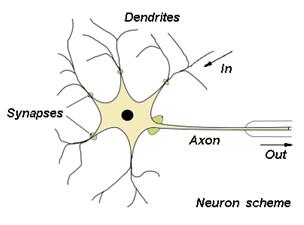
\includegraphics[scale=0.9]{gambar/neuron.jpg}
      % Keterangan gambar yang diinputkan
      \caption{Sistem Neuron Pada Otak manusia (Sumber: socs.binus.ac.id)}
      % Label referensi dari gambar yang diinputkan
      \label{fig:MechineLearning}
    \end{figure}\\
    mengikut pada gambar diatas, ada beberapa bagian otak manusia:
    \begin{enumerate}[nolistsep]
      \item Dendrit (Dendrites) berfungsi untuk mengirimkan impuls yang diterima ke badan sel syaraf.
      \item Akson (Axon) berfungsi untuk mengirimkan impuls dari badan sel ke jaringan lain
      \item Sinapsis berfungsi sebagai unit fungsional di antara dua sel syaraf.
    \end{enumerate}
\end{enumerate}

